\RCS$Revision: 207461 $
\RCS$HeadURL: svn+ssh://snarayan@svn.cern.ch/reps/tdr2/notes/IN-14-XXX/trunk/IN-14-XXX.tex$
\RCS$Id: IN-14-XXX.tex 207461 2013-09-18 14:56:50Z tapper $
\newcommand{\Na}{N_\text{accesses}}
\newcommand{\Nf}{N_\text{files}}
\newcommand{\Nr}{\langle N_\text{replicas}\rangle}
\newlength\cmsFigWidth
\ifthenelse{\boolean{cms@external}}{\setlength\cmsFigWidth{0.85\columnwidth}}{\setlength\cmsFigWidth{0.4\textwidth}}
\ifthenelse{\boolean{cms@external}}{\providecommand{\cmsLeft}{top}}{\providecommand{\cmsLeft}{left}}
\ifthenelse{\boolean{cms@external}}{\providecommand{\cmsRight}{bottom}}{\providecommand{\cmsRight}{right}}
\input{commands.tex}
\cmsNoteHeader{IN 2014/XXX}

\title{Disk Storage Usage and Metrics for Dynamic Data Management}
\address[MIT]{Massachusetts Institute of Technology}
\author[MIT]{S. Narayanan}
\author[MIT]{M. Goncharov}
\author[MIT]{C. Paus}

\hypersetup{%
pdfauthor={S. Narayanan, M. Goncharov, C. Paus},%
pdftitle={Disk Storage Usage and Metrics for Dynamic Data Management},%
pdfsubject={CMS},%
pdfkeywords={CMS, Dynamic Data Management, popularity}%
}

\date{\today}

\abstract{
%%
  In the CMS experiment, detector and Monte Carlo simulation data are ordered in
  datasets, which have some common properties and are usually analyzed as a
  whole.  The popularity of such datasets varies substantially, which opens the
  question how to best distribute the datasets such that they are optimally
  accessible at the various computing sites. Generally speaking, popular
  datasets should be replicated at several sites while less popular datasets
  might just have a single copy in the overall system. Also as the data taking
  progresses and new Monte Carlo simulation datasets become available, those
  datasets have to be distributed in the system and outdated datasets have to be
  removed. The Dynamic Data Management tools automatically manage the
  replication of datasets in the distributed multi-site computing system with
  the goal of optimising the system performance. In this note, we describe a
  metric for the performance of Dynamic Data Management, based on the number
  of user accesses of a the given datasets.
%%
}

\maketitle %maketitle comes after all the front information has been supplied

\tableofcontents

%+++++++++++++++++++++++++++++++++++++++++++++++++++++++++++++++++++++++++++++++
\section{Introduction}\label{sec:introduction}

Dynamic Data Management currently manages a pool of approximately 20~PB across
several Tier-2 and Tier-1 sites. The purpose of the management to first order is
the creation and deletion of replicas of datasets that are part of the pool.
Additional replicas of a dataset are created when the dataset is particular
popular while excess replicas are deleted when they are less popular. The
creation and deletion of replicas does not add new datasets to the pool nor does
it remove datasets entirely from it. Adding new datasets to the pool and
completely removing datasets from it is treated separately. Newly created
datasets that are relevant to the Physics Group get automatically added to the
pool by the Computing Operations group and datasets will be deleted following
deletion campaigns that are driven by the Physics Groups in the experiment.
This means usually for a given dataset there is at least one copy in the system
often referred to as the last copy. If a dataset is declared deprecated, all
copies will be deleted.

A good measure of the performance of the algorithms used to create and delete
dataset replicas is the number of accesses per replica. If, for a given dataset,
this number is very large, then the dataset is not sufficiently replicated. On
the other hand, if it is very small for many datasets, then we are maintaining
too many replicas of unused datasets. To produce plots of the popularity of
datasets in a given time interval we have to carefully determine the list of
datasets that we have to consider and determine four attributes for each
dataset: number of accesses, size on disk, number of files, and average number
of replicas.

The plot provides a measure of how well our computing system is using the given
disk space in our data pool. In the following we explain in detail how we
determine the list of datasets we consider and how we calculate the four above
listed properties for each dataset.

%+++++++++++++++++++++++++++++++++++++++++++++++++++++++++++++++++++++++++++++++
\section{Ingredients}

%===============================================================================
\subsection{Dataset selection}

The CMS experiment creates a large number of datasets of which not all are
commonly used by the people doing analysis. From the detector we have RAW and
RECO data formats, but since 2011 the much more compressed AOD datasets had been
established as the datasets used for analysis. The other data formats are mostly
stored on tape and are used for production purposes when the data or Monte Carlo
simulation samples get re-reconstructed with better calibrations/alignments
and/or new reconstruction algorithms. The majority of data on the Tier-2 centers
are therefore of AOD or AODSIM format or since recently the even more reduced
MINIAOD and MINIAODSIM format, but there are some other formats. In this study
we evaluate data popularity in a given time interval and distinguish between two
scenarios for the selection of datasets to consider.
%
\begin{itemize}
\item include all datasets that are managed by phedex~\ref{PHEDEX} in any of the
   official data groups and that were at some point during the considered
   interval at a Tier-2 site, or
\item include all datasets that are or were in the past managed by
   phedex~\ref{PHEDEX} in the 'AnalysisOps' data group (this is the dynamic
   data management pool) and that were at some point during the considered
   interval at a Tier-2 site.
\end{itemize}

We distinguish these two scenarios because the first one very generally shows
the usage of our entire storage, while the second scenario zooms in on the
dynamically managed data pool, and thus offers itself as a tool to optimize the
data distribution for the best system performance.

While the dataset selection appears to be a straight forward the fact that we do
not have a full record of the contents of the data storage of the order 50
Tier-2 sites makes it complicated. Obtaining the list of relevant datasets is a
non trivial issue. In the popularity database we can easily find all datasets
that were used at a particular site in the given time interval, but datasets
that were not accessed during this time interval are not recorded and therefore
we must use an alternative source to find all datasets.

%===============================================================================
\subsection{Average $N_\text{replicas}$}

Phedex directly provides us with the current locations of all datasets. However,
this information is not directly available for the past. Thus, Phedex transfer
and deletion histories are used to infer the timeline of the presence of a
dataset on a given site.

The histories are `sanitized' to remove self-inconsistent entries such as the
transfer of a dataset to a site on which it already exists. It is assumed that
each site can only contain one copy of a dataset. If there is no Phedex history
for a given dataset on a given site, but we know that the dataset is currently
on that site, then it is assumed to have existed on the site since its creation
time which is determined using DAS.

Having collected this information, $\Nr$ can be computed for a given time
interval $[t_0,t_1]$. Then, summing over the sites:
%
\begin{equation}
  \Nr = \sum_{S\in \text{sites}} \dfrac{\text{time on }S
        \text{ during }[t_0,t_1]}{t_1-t_0}
\end{equation}
%
This gives the average number of replicas of a dataset in a specific time
interval. If a dataset was not at the site for the entire considered time
interval the count is prorated with the fraction of time it was present in the
interval.

%===============================================================================
\subsection{Number of Accesses $\Na$ and File $N_\text{files}$,
            and Size $\text{size}$}

The remaining variables are relatively easily calculated. The number of files
and size of a dataset are retrieved from DAS. It should be noted that we assume
each replica is a ``full'' replica. An incomplete replica may be missing files
and consequently it will have a smaller size. We compute $\Na$ using the caches
maintained by Detox. Detox is the Dynamic Data Management tool which deals with
the deletion of deprecated datasets and under-utilized replicas. In order to
make the latter decision, Detox keeps a local record of the number of accesses
made to each replica of each dataset, derived from the popularity API. $\Na$ for
a dataset is defined as the total number of accesses over all replicas of that
dataset.

%+++++++++++++++++++++++++++++++++++++++++++++++++++++++++++++++++++++++++++++++
\section{Filling the plot}

%===============================================================================
\subsection{Dataset selection}

We consider all datasets that are currently on, or have been on, Tier 2 sites
(Tier-1s are excluded). This information is gathered from two places. First, we
ask Phedex for all datasets which are currently on Tier-2s. Then, we use the
\verb|deleterequests| Phedex API to determine all datasets which have been
deleted during the relevant time interval. We consider all datasets in the union
of these two sets. Finally, we double-check using the Phedex transfer/deletion
histories that it actually was on at least one site during the interval. If the
dataset passes this check, a corresponding entry is made in the histogram, as
discussed below.

%===============================================================================
\subsection{Binning}

Having computed these variables for each dataset, the popularity plot may be
made. The histogram is filled for each dataset by choosing the following
bin-value:
%
\begin{equation}
  \dfrac{N_\text{accesses}}{N_\text{files}\cdot \Nr}
\end{equation}
%
The factor of $\Nf$ in the denominator is due to the fact that a single request
to a dataset actually consists of a series of requests to each file in the
dataset. Dividing by $N_\text{files}$ ensures that this quantity is the same for
small and large datasets. The entry is given weight:
%
\begin{equation}
  \Nr\cdot \text{size}
\end{equation}
%
For ease of comparing plots made under different conditions, the bin-value is
normalized to the length of the time interval (in Figure~\ref{fig:usage}, the unit of time is
months). Finally, the plot is normalized to have an integral of unity. The
un-normalized integral can be thought of as a measure of ``average data volume''
during the interval, since it can be computed as:
%
\begin{equation}
  \sum_\text{datasets} \Nr \cdot \text{size}
\end{equation}
%
Finally, it should be noted that there are two special bins in
Figure~\ref{fig:usage}. The very last bin is the overflow bin. The very first
bin contains those entries for which $\Na=0$ exactly. It is important to recall
that the histogram is only filled with datasets that were on at least one site
during the relevant interval. Thus, the very first bin shows the fractional
volume of datasets which were on disk, but not accessed, during an interval.

\begin{figure}[h!]
  \centering
  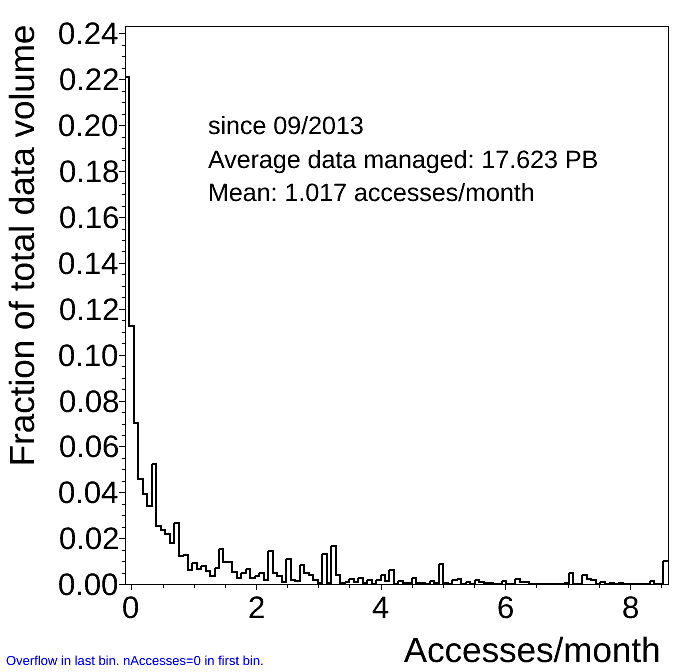
\includegraphics[width=0.45\textwidth]{plots/analysisOps_usage.png}~ 
  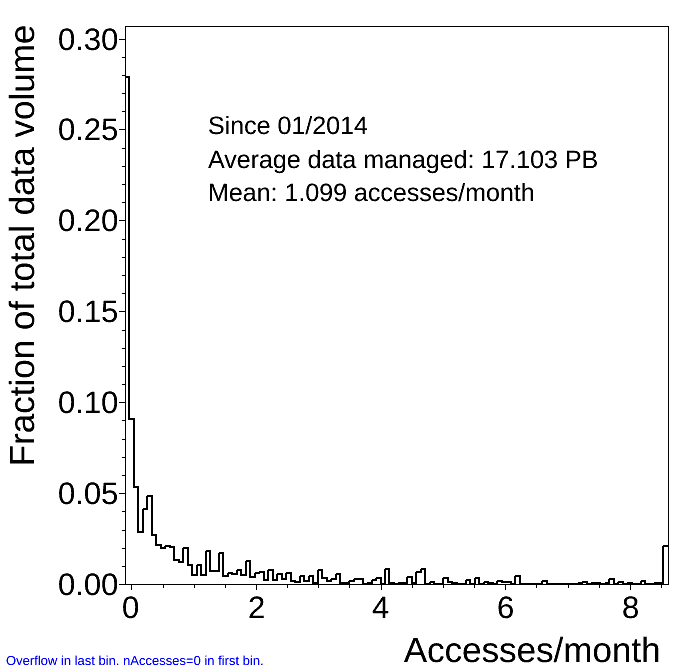
\includegraphics[width=0.45\textwidth]{plots/DatasetSummary01-2014_nSitesAverage.png}\\
  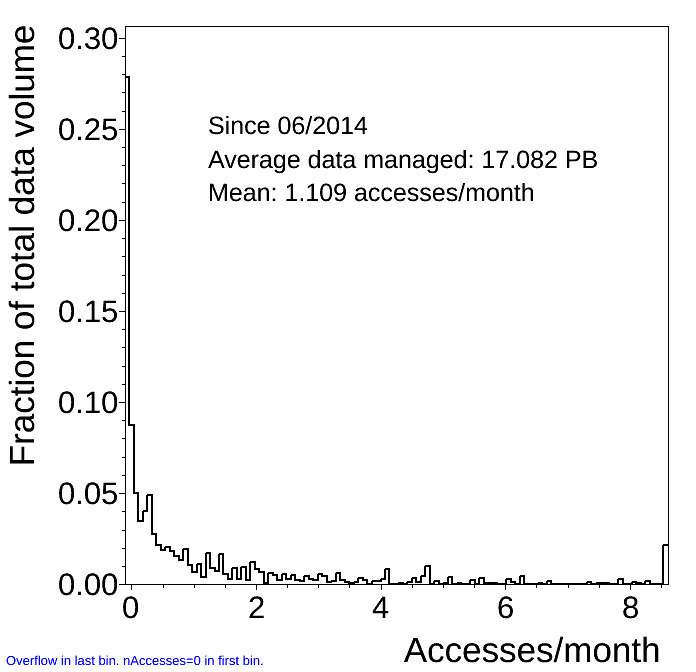
\includegraphics[width=0.45\textwidth]{plots/DatasetSummary06-2014_nSitesAverage.png}~
  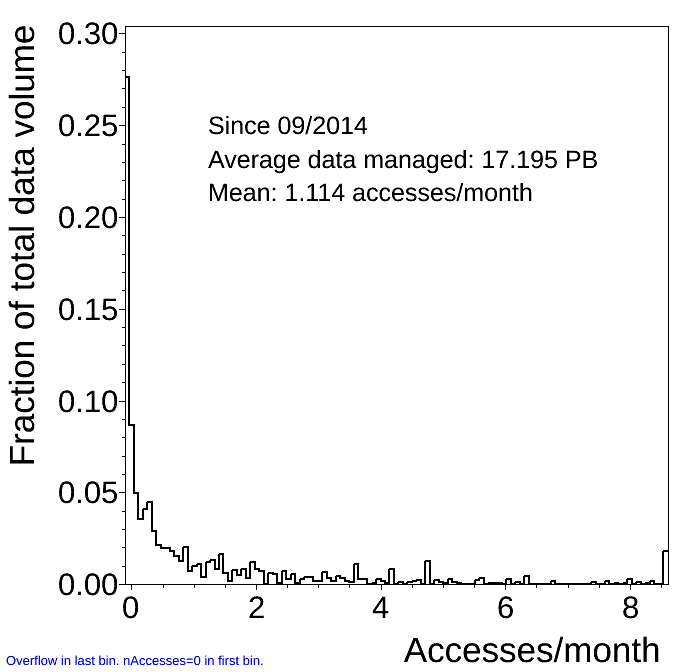
\includegraphics[width=0.45\textwidth]{plots/DatasetSummary09-2014_nSitesAverage.png}
  \caption{Usage plots datasets in AnalysisOps for various time intervals.}
  \label{fig:usage}
\end{figure}

\clearpage
%% % >> acknowledgements (for journal papers)
%% % Please include the latest version from https://twiki.cern.ch/twiki/bin/viewauth/CMS/Internal/PubAcknow.
%% \section*{Acknowledgements}
%% We congratulate our colleagues in the CERN accelerator departments for the
%% excellent performance of the LHC and thank the technical and administrative
%% staffs at CERN and at other CMS institutes for their contributions to the
%% success of the CMS effort. In addition, we gratefully acknowledge the computing
%% centres and personnel of the Worldwide LHC Computing Grid for delivering so
%% effectively the computing infrastructure essential to our analyses. Finally, we
%% acknowledge the enduring support for the construction and operation of the LHC
%% and the CMS detector provided by the following funding agencies: BMWFW and FWF
%% (Austria); FNRS and FWO (Belgium); CNPq, CAPES, FAPERJ, and FAPESP (Brazil); MES
%% (Bulgaria); CERN; CAS, MoST, and NSFC (China); COLCIENCIAS (Colombia); MSES and
%% CSF (Croatia); RPF (Cyprus); MoER, ERC IUT and ERDF (Estonia); Academy of
%% Finland, MEC, and HIP (Finland); CEA and CNRS/IN2P3 (France); BMBF, DFG, and HGF
%% (Germany); GSRT (Greece); OTKA and NIH (Hungary); DAE and DST (India); IPM
%% (Iran); SFI (Ireland); INFN (Italy); NRF and WCU (Republic of Korea); LAS
%% (Lithuania); MOE and UM (Malaysia); CINVESTAV, CONACYT, SEP, and UASLP-FAI
%% (Mexico); MBIE (New Zealand); PAEC (Pakistan); MSHE and NSC (Poland); FCT
%% (Portugal); JINR (Dubna); MON, RosAtom, RAS and RFBR (Russia); MESTD (Serbia);
%% SEIDI and CPAN (Spain); Swiss Funding Agencies (Switzerland); MST (Taipei);
%% ThEPCenter, IPST, STAR and NSTDA (Thailand); TUBITAK and TAEK (Turkey); NASU and
%% SFFR (Ukraine); STFC (United Kingdom); DOE and NSF (USA).

%% **DO NOT REMOVE BIBLIOGRAPHY**
\bibliography{auto_generated}   % will be created by the tdr script.
%%% DO NOT ADD \end{document}!
